%%%%%%%%%%%%%%%%%%%%%%%%%%%%%%%%%%%%%%%%%
% University/School Laboratory Report
% LaTeX Template
% Version 3.1 (25/3/14)
%
% This template has been downloaded from:
% http://www.LaTeXTemplates.com
%
% Original author:
% Linux and Unix Users Group at Virginia Tech Wiki 
% (https://vtluug.org/wiki/Example_LaTeX_chem_lab_report)
%
% License:
% CC BY-NC-SA 3.0 (http://creativecommons.org/licenses/by-nc-sa/3.0/)
%
%%%%%%%%%%%%%%%%%%%%%%%%%%%%%%%%%%%%%%%%%

%----------------------------------------------------------------------------------------
%	PACKAGES AND DOCUMENT CONFIGURATIONS
%----------------------------------------------------------------------------------------

\documentclass{article}

\usepackage{graphicx} % Required for the inclusion of images
\usepackage{amsmath} % Required for some math elements 

\setlength\parindent{0pt} % Removes all indentation from paragraphs

\renewcommand{\labelenumi}{\alph{enumi}.} % Make numbering in the enumerate environment by letter rather than number (e.g. section 6)

%\usepackage{times} % Uncomment to use the Times New Roman font

%----------------------------------------------------------------------------------------
%	DOCUMENT INFORMATION
%----------------------------------------------------------------------------------------

\title{Using Reinforcement Learning \\ to solve the pendulum swing up} % Title

\author{Bruno \textsc{Costa}} % Author name

\date{\today} % Date for the report

\begin{document}

\maketitle % Insert the title, author and date

% If you wish to include an abstract, uncomment the lines below
% \begin{abstract}
% Abstract text
% \end{abstract}

%----------------------------------------------------------------------------------------
%	SECTION 1
%----------------------------------------------------------------------------------------

\section{Objective}

We want to solve the pendulum swing-up problem [Figure \ref{fig:swing}] using Reinforcement Learning techiniques, more specifically, using Actor-Critic framework. For that, we will consider both action and state space as continuos, and for such, we will need to use a Function Approximator (FA) for them both. The FA we will use is the tile coding. For the sake of organization, we will split our goal in two:

\begin{figure}[h!]
    \centering
    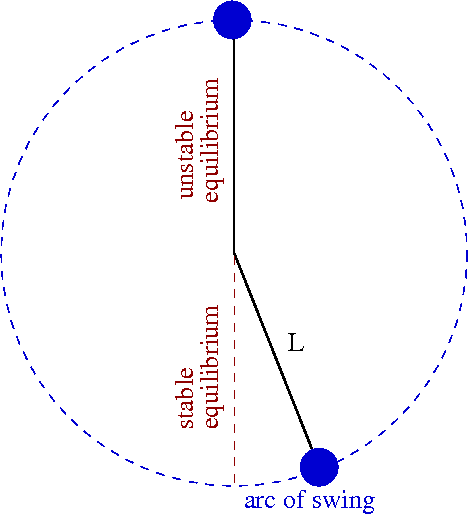
\includegraphics[width=.4\textwidth]{swing.png}
    \caption{The Pendulum Swing-up problem}
    \label{fig:swing}
\end{figure}

% If you have more than one objective, uncomment the below:
\begin{description}
\item[Solve the pendulum balancing] \hfill \\
In this scenario, the pendulum start on top, and our policy must only balancing it there.
\item[Swing-up] \hfill \\
Finally, in this scenario, we will consider the full problem, starting the pendulum on the bottom.
\end{description}

%----------------------------------------------------------------------------------------
%	SECTION 2
%----------------------------------------------------------------------------------------

\section{Pendulum Balancing}
For the balancing, we changed the code and created a new environment, in which the first observation is $[\pi,0]$.
Using the attributes listed in Table \ref{tab:balancing} we could make it as we can see in Figures \ref{fig:cr_balancing}, \ref{fig:actor_balancing} and \ref{fig:critic_balancing}.

\begin{table}
    \centering
    \begin{tabular}{ll}
    \multicolumn{2}{c}{Actor}   \\ \hline
    $\alpha$       & $0.005$    \\
    \multicolumn{2}{c}{Critic}   \\ \hline
    $\alpha$       & $0.1$      \\
    \multicolumn{2}{c}{Parameter}   \\ \hline
    $\gamma$       & $0.97$     \\
    $\lambda$      & $0.67$     \\
    $\sigma$       & $1.0$      \\
    \end{tabular}
    \caption{Parameters used in Pendulum Balancing}
    \label{tab:balancing}
\end{table}

\begin{figure}[h!]
    \centering
    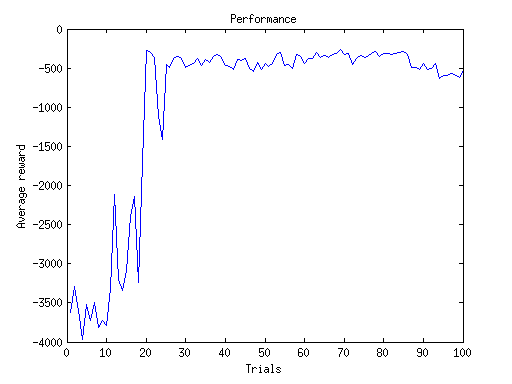
\includegraphics[width=.7\textwidth]{cr_balancing.png}
    \caption{Total reward for each trial in the balacing problem}
    \label{fig:cr_balancing}
\end{figure}

\begin{figure}[h!]
    \centering
    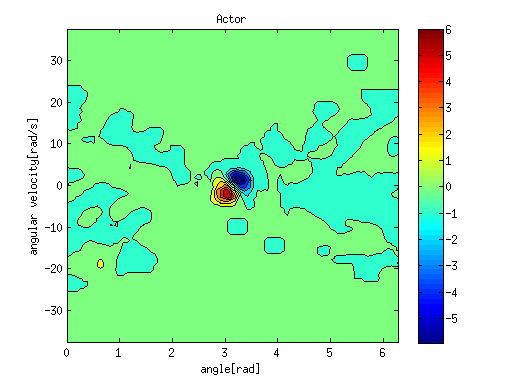
\includegraphics[width=.7\textwidth]{actor_balancing.png}
    \caption{The Actor for the balancing problem}
    \label{fig:actor_balancing}
\end{figure}

\begin{figure}[h!]
    \centering
    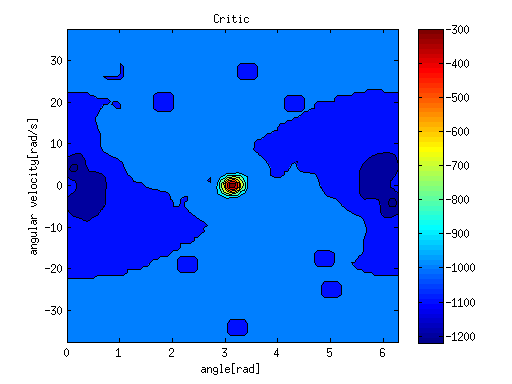
\includegraphics[width=.7\textwidth]{critic_balancing.png}
    \caption{The Critic for the balancing problem}
    \label{fig:critic_balancing}
\end{figure}

\begin{figure}[h!]
    \centering
    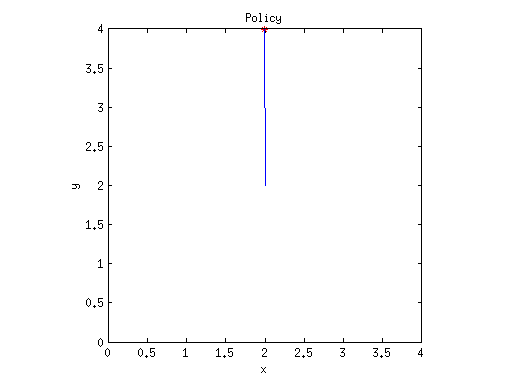
\includegraphics[width=.7\textwidth]{result_balancing.png}
    \caption{The final position for the balancing problem}
    \label{fig:result_balancing}
\end{figure}

As we can see, it works(Figure \ref{fig:result_balancing}). In Figure \ref{fig:cr_balancing} we can see that the average reward is good after 30 trials, Another interesting thing to notice is the policy in Figure \ref{fig:actor_balancing}: as the angle goes to the left, the action is to push to the right and vice-versa. The critic, in Figure \ref{fig:critic_balancing} shows that the central position is the best.

%----------------------------------------------------------------------------------------
%	SECTION 3
%----------------------------------------------------------------------------------------

\section{Pendulum Swing-up}
For the swing-up, we used the environment as it is. The first observation is $[0,0]$.
Using the attributes listed in Table \ref{tab:swing} (the same attributes here used in the balancing) we could make it as we can see in Figures \ref{fig:cr_swing}, \ref{fig:actor_swing} and \ref{fig:critic_swing}.

\begin{table}
    \centering
    \begin{tabular}{ll}
    \multicolumn{2}{c}{Actor}   \\ \hline
    $\alpha$       & $0.005$    \\
    \multicolumn{2}{c}{Critic}   \\ \hline
    $\alpha$       & $0.1$      \\
    \multicolumn{2}{c}{Parameter}   \\ \hline
    $\gamma$       & $0.97$     \\
    $\lambda$      & $0.67$     \\
    $\sigma$       & $1.0$      \\
    \end{tabular}
    \caption{Parameters used in Pendulum Swing-up}
    \label{tab:balancing}
\end{table}

\begin{figure}[h!]
    \centering
    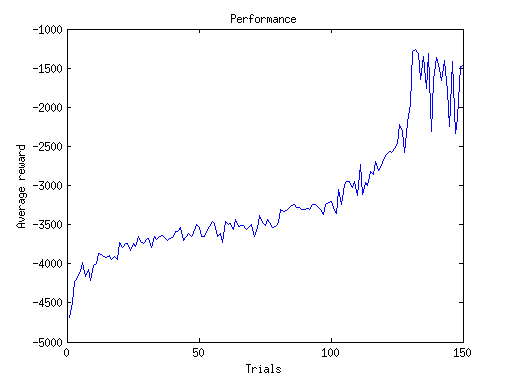
\includegraphics[width=.7\textwidth]{cr_swing.png}
    \caption{Total reward for each trial in the swing-up problem}
    \label{fig:cr_swing}
\end{figure}

\begin{figure}[h!]
    \centering
    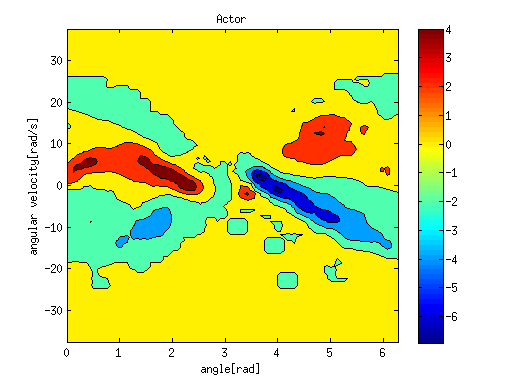
\includegraphics[width=.7\textwidth]{actor_swing.png}
    \caption{The Actor for the swing problem}
    \label{fig:actor_swing}
\end{figure}

\begin{figure}[h!]
    \centering
    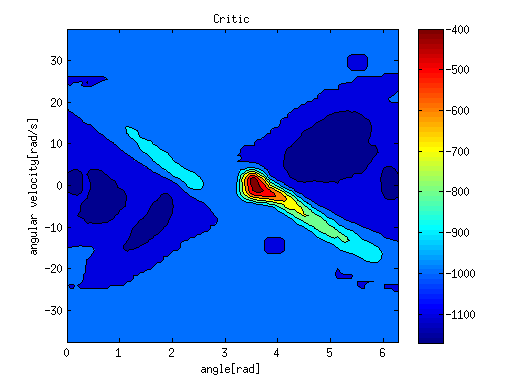
\includegraphics[width=.7\textwidth]{critic_swing.png}
    \caption{The Critic for the swing problem}
    \label{fig:critic_swing}
\end{figure}

\begin{figure}[h!]
    \centering
    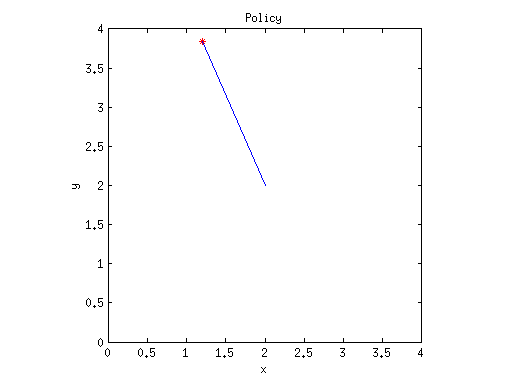
\includegraphics[width=.7\textwidth]{result_swing.png}
    \caption{The final position for the swing problem}
    \label{fig:result_swing}
\end{figure}

As we can see, it also works(Figure \ref{fig:result_swing}). In Figure \ref{fig:cr_swing} we can see that the average reward is good after 130 trials, which is much more than the balancing problem. Another interesting thing to notice is the policy in Figure \ref{fig:actor_swing}: there is the swinging, and then, once the pole is on top, it has to balance. The critic, in Figure \ref{fig:critic_swing} shows that the central position is the best.


%----------------------------------------------------------------------------------------
%	SECTION 4
%----------------------------------------------------------------------------------------

\section{Difficulties}
My first version was updating the wrong state, and because of that, it wasn't converging. For each transition, we have the old state (s), the action we took (a), the new state (s') and the reward we get (r). We must update s not s'.

%----------------------------------------------------------------------------------------
%	BIBLIOGRAPHY
%----------------------------------------------------------------------------------------

\bibliographystyle{apalike}
\bibliography{sample}

%----------------------------------------------------------------------------------------


\end{document}
